% -*- coding: utf-8 -*-
% ビルド: tectonic -X compile AND_SCREENING_EXPLAINER_v1.tex
% 図: and_figures/*.png (scripts/make_and_figures.py で生成)
% 数値の出どころ: and_feasibility.json / and_frontier.json / and_backtest.json
\documentclass[a4paper,10.5pt]{article}

\usepackage{xeCJK}
\setmainfont{TeX Gyre Termes}
\setsansfont{TeX Gyre Heros}
\setCJKmainfont{Noto Serif CJK JP}
\setCJKsansfont{Noto Sans CJK JP}
\XeTeXlinebreaklocale "ja"
\XeTeXlinebreakskip=0pt plus 1pt
% 丸数字(①②③④)・罫線(─)・幾何記号は欧文フォントに無いので CJK 側で組む
\xeCJKDeclareCharClass{CJK}{"2460 -> "24FF, "2500 -> "257F, "25A0 -> "25FF}

\usepackage[a4paper,left=22mm,right=22mm,top=20mm,bottom=22mm]{geometry}
\usepackage{setspace}
\setstretch{1.18}
\setlength{\parindent}{0pt}
\setlength{\parskip}{0.55em}

\usepackage{amsmath,amssymb}
\usepackage{graphicx}
\usepackage{booktabs}
\usepackage{array}
\usepackage{caption}
\usepackage{xcolor}
\usepackage{enumitem}
\usepackage{titlesec}
\usepackage{fancyhdr}
\usepackage[hidelinks]{hyperref}
\usepackage[most]{tcolorbox}

\definecolor{navy}{HTML}{1F4E79}
\definecolor{warn}{HTML}{AA3333}
\definecolor{lightg}{HTML}{F2F4F7}
\definecolor{rulec}{HTML}{C8CDD4}

\captionsetup{font=small,labelfont={bf,color=navy},skip=4pt}
\titleformat{\section}{\sffamily\large\bfseries\color{navy}}{\thesection.}{0.6em}{}
\titleformat{\subsection}{\sffamily\normalsize\bfseries\color{navy}}{}{0em}{}
\titlespacing{\section}{0pt}{1.4em}{0.5em}
\titlespacing{\subsection}{0pt}{0.9em}{0.3em}

\pagestyle{fancy}\fancyhf{}
\fancyhead[L]{\footnotesize\sffamily\color{navy}なぜ「守る堀→破る堀→離れる堀」の順番スクリーニングでは20社を選べないのか}
\fancyhead[R]{\footnotesize\sffamily\thepage}
\renewcommand{\headrulewidth}{0.4pt}

\newtcolorbox{keybox}[1][]{colback=lightg,colframe=navy,boxrule=0.9pt,arc=2pt,
  left=8pt,right=8pt,top=7pt,bottom=7pt,#1}
\newtcolorbox{termbox}[1][]{colback=white,colframe=rulec,boxrule=0.7pt,arc=2pt,
  left=8pt,right=8pt,top=6pt,bottom=6pt,#1}
\newtcolorbox{warnbox}[1][]{colback=white,colframe=warn,boxrule=0.9pt,arc=2pt,
  left=8pt,right=8pt,top=7pt,bottom=7pt,#1}

\newcommand{\jt}[1]{\textsf{\bfseries\color{navy}#1}}

\begin{document}

\thispagestyle{empty}
\begin{center}
{\sffamily\bfseries\color{navy}\LARGE なぜ「守る堀 $\rightarrow$ 破る堀 $\rightarrow$ 離れる堀」の\\[2pt]
順番スクリーニングでは20社を選べないのか}\\[10pt]
{\sffamily\large ── 初学者向け解説 ──}\\[14pt]
{\small 2026年7月28日\hspace{1.5em}／\hspace{1.5em}検証の正典: \texttt{AND\_SCREENING\_FEASIBILITY\_v1.md}}
\end{center}

\vspace{4pt}

\begin{keybox}
{\sffamily\bfseries\color{navy}この資料が答えること}\\[3pt]
チームからいただいた提案は、こういうものでした。

\begin{quote}
「守る堀でスクリーニングして、次に破る堀でスクリーニングして、次に離れる堀でスクリーニングする。
そうすれば全部の要素を持った最強の20社が選べるのでは?」
\end{quote}

とても筋の通ったアイデアです。実際のデータで試しました。\textbf{結論は「できない」}でした。
この資料は、その理由を4つに分けて、数字と絵で説明します。予備知識はいりません。
\end{keybox}

\begin{keybox}[colback=white,colframe=warn]
{\sffamily\bfseries\color{warn}結論（3行）}
\begin{enumerate}[leftmargin=1.4em,itemsep=2pt,topsep=3pt]
\item 「同じ業種は2社まで」という分散のルールを守る限り、ふるいをどれだけ緩めても\textbf{最大16社}しか組めません。
\item 業種のルールを緩めれば20社は組めますが、業種の数が13$\rightarrow$6に減り、\textbf{4つの物差しすべてで現行の20社に届きません}。
\item そもそも3段目の「離れる堀のふるい」は、\textbf{会社ではなく業種を判定しているだけ}でした。だから「3つ全部通ったから最強」という理屈が成り立ちません。
\end{enumerate}
\end{keybox}

\vfill
{\footnotesize
本資料の数値はすべて実際のデータ（東証上場3,649社・2026年4月末時点）を計算した結果です。
再現方法は付録Bに書きました。なお成績（リターン）はSTOCKリーグの採点対象外であり、
本資料は「提案が実行可能かどうか」の判定に限った資料です。\par}

\newpage

%=====================================================================
\section{提案の中身を、絵で見る}

まず、提案されたやり方を絵にします。会社の集まりを、3枚のふるいに順番にかけていきます。

\begin{figure}[h]
\centering
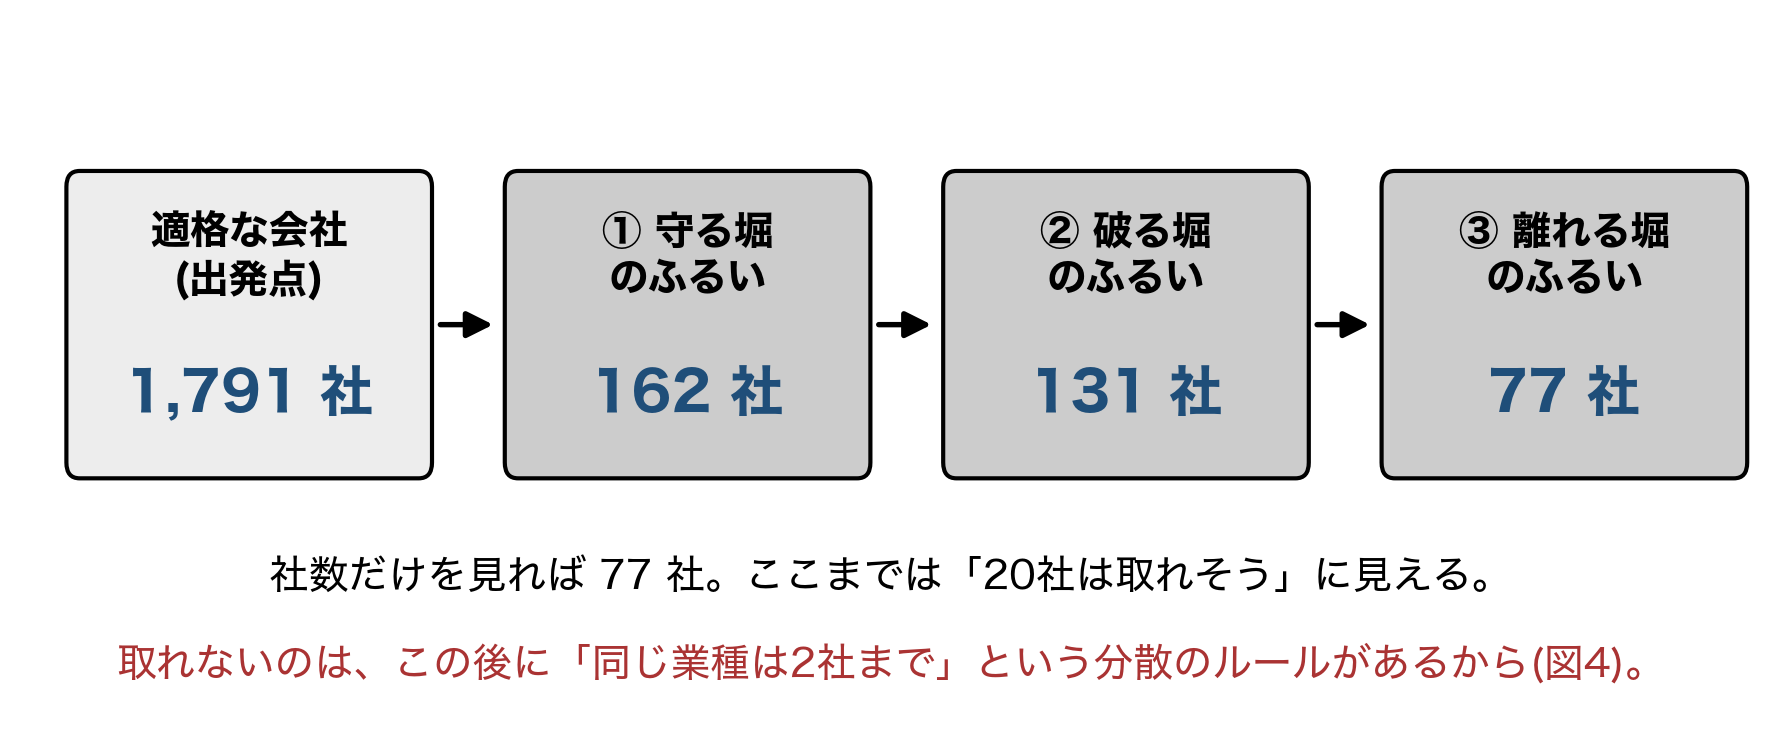
\includegraphics[width=\linewidth]{and_figures/f1_funnel.png}
\caption{提案どおりに3枚のふるいを順番にかけた結果（実測）}
\end{figure}

出発点の\jt{1,791社}は、金融を除き、上場廃止の恐れがなく、毎日そこそこ売買されていて、
過去3年分の株価が揃っている会社です。ここから、

\begin{itemize}[leftmargin=1.4em,itemsep=1pt,topsep=2pt]
\item \jt{① 守る堀のふるい}：もうけが厚くて財務が丈夫な会社を残す（ＲＯＥ15\%以上・営業利益率10\%以上・自己資本比率50\%以上・3期赤字なし・増収増益など）$\rightarrow$ \textbf{162社}
\item \jt{② 破る堀のふるい}：割安に放置されていて、これから変わりそうな会社を残す $\rightarrow$ \textbf{131社}
\item \jt{③ 離れる堀のふるい}：ＡＩ・半導体などの新しい波に乗る会社を残す $\rightarrow$ \textbf{77社}
\end{itemize}

77社残っています。だから一見「ここから20社選べばいいじゃないか」と思えます。
\textbf{ところが選べません。}理由を順番に見ていきます。

%=====================================================================
\section{言葉の準備（3つだけ）}

\begin{termbox}
\jt{ふるい（スクリーニング）}\quad 条件を決めて、通った会社だけ残す作業のこと。
「ＲＯＥが15\%以上」なら、それ未満の会社は全部落ちます。

\medskip
\jt{ＡＮＤ（かつ）}\quad 「①も②も③も全部通った会社だけ残す」というつなぎ方。
提案されているのはこれです。反対に「①か②か③のどれかで良い」は\jt{ＯＲ（または）}で、
現行のやり方はこちらに近い（役割ごとに別々に選ぶ）。

\medskip
\jt{業種上限（同じ業種は2社まで）}\quad 現行の分散ルールです。
20社が全員半導体だと、半導体が転けたときに全部やられます。
それを防ぐため「同じ業種からは最大2社」と決めています。
\end{termbox}

この3つ目が、今回の話の主役になります。

%=====================================================================
\section{理由① ＡＮＤは掛け算なので、絞れる強さに天井ができる}

\subsection{たとえ話}

学校で「身長が高い上位30\%」「足が速い上位30\%」「テストが上位30\%」の3つを全部満たす人を探すとします。
3つがバラバラ（互いに関係ない）なら、残るのはだいたい
$0.3 \times 0.3 \times 0.3 = 0.027$、つまり\textbf{全体の2.7\%}です。
1000人の学校なら27人。ふるいを「上位10\%」に厳しくすると
$0.1^3 = 0.001$で\textbf{1人}になってしまいます。

\jt{ＡＮＤは掛け算}です。ふるいを重ねるほど、残る人数は掛け算で減ります。

\subsection{今回のデータで確かめる}

三つの点数（守る堀・破る堀・離れる堀）は、実測でほとんど互いに関係がありませんでした。
順位の相関は、守×破が$+0.05$、守×離が$+0.01$、破×離が$-0.06$。
どれもほぼ0、つまり\textbf{たとえ話とほぼ同じ「バラバラ」の状況}です。

\begin{figure}[h]
\centering
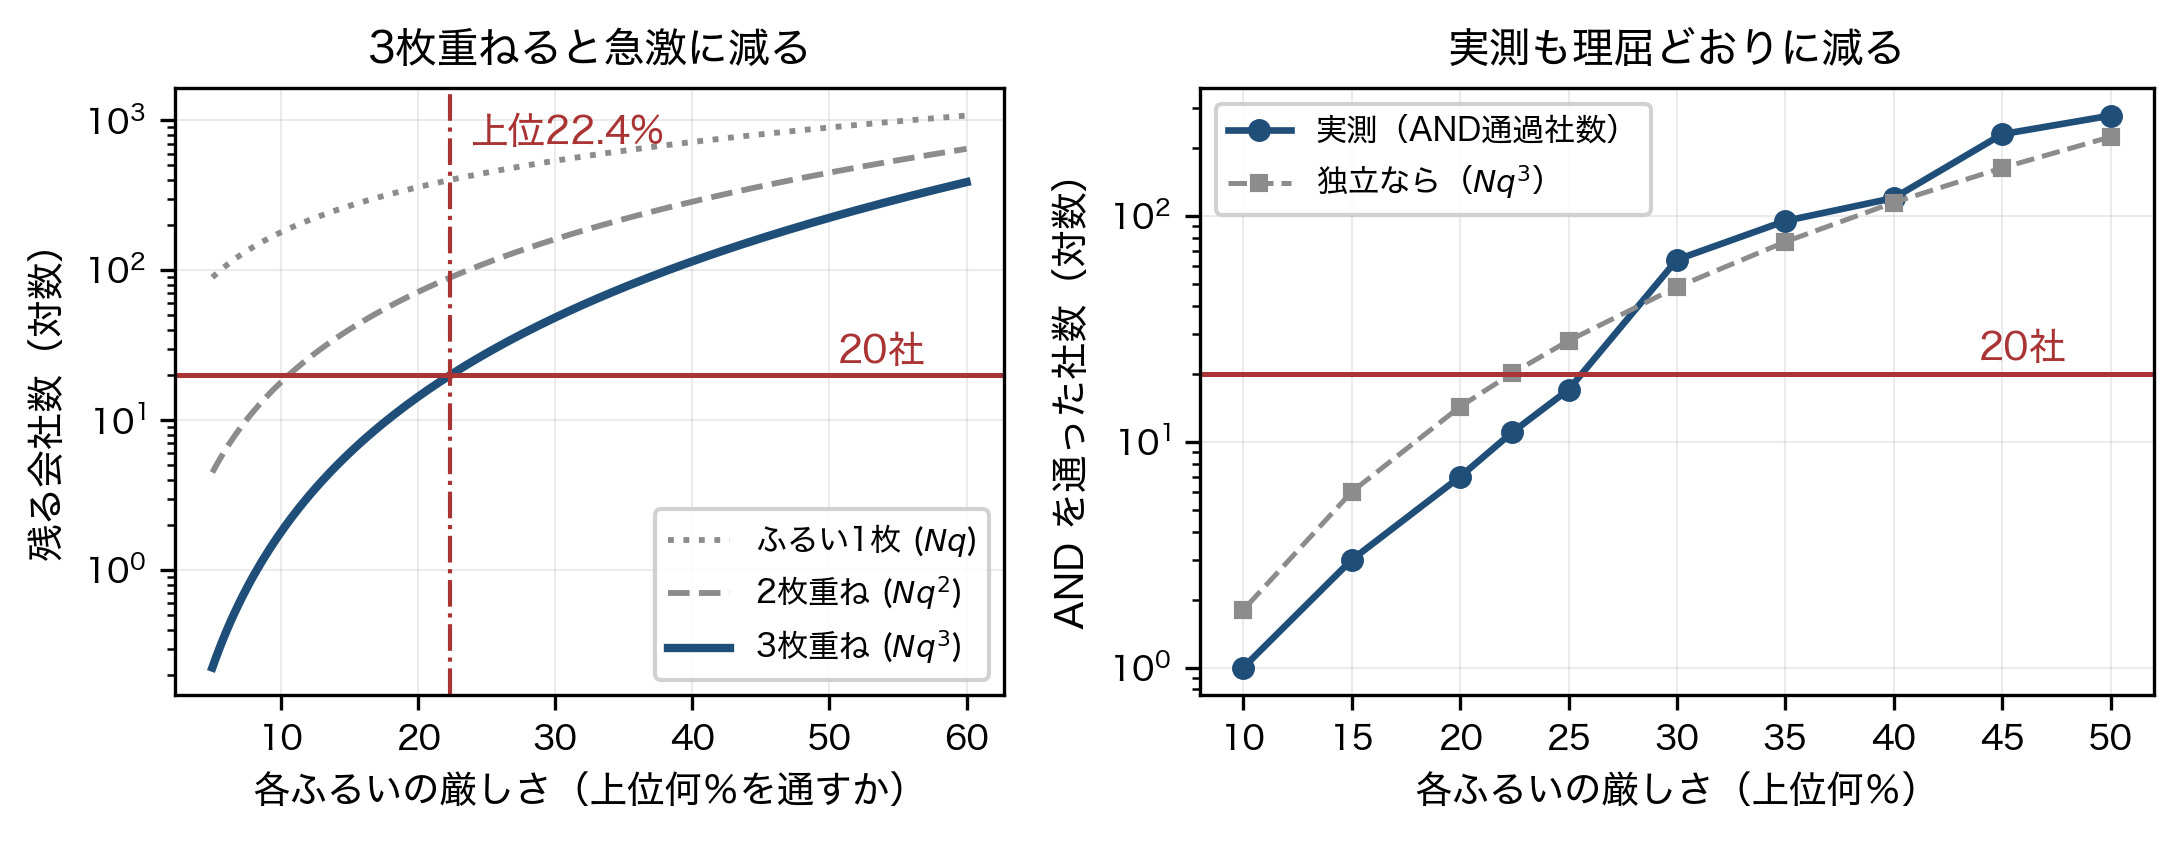
\includegraphics[width=\linewidth]{and_figures/f2_multiply.png}
\caption{左：理屈のうえでの減り方。右：実測。どちらも同じように急落する}
\end{figure}

ここから、逆算ができます。出発点1,791社から20社を残すには、
$1791 \times q^3 = 20$ を解いて $q = 0.224$。つまり

\begin{warnbox}
\jt{各ふるいを「上位22\%」より厳しくすると、20社に届かなくなる。}\\
言いかえると、\textbf{ＡＮＤ方式では「3つ全部でエリート」を要求できません}。
どのふるいも「上位2割くらい」までしか絞れないのです。
\end{warnbox}

対して現行のやり方は、守る堀だけで162社（上位9.0\%）まで絞り、そこから5社（\textbf{上位0.28\%}）を選んでいます。
\textbf{役割を分けているからこそ、各層で深く絞れる}という関係になっています。

%=====================================================================
\section{理由② 三層の「一番良い会社」は、それぞれ別の会社だった}

「3つ全部で優秀な会社」がたくさんいれば、ＡＮＤは成立します。実際に調べました。
守る堀の点数トップ20、破る堀のトップ20、離れる堀のトップ20を並べて、
重なっている会社を数えます。

\begin{figure}[h]
\centering
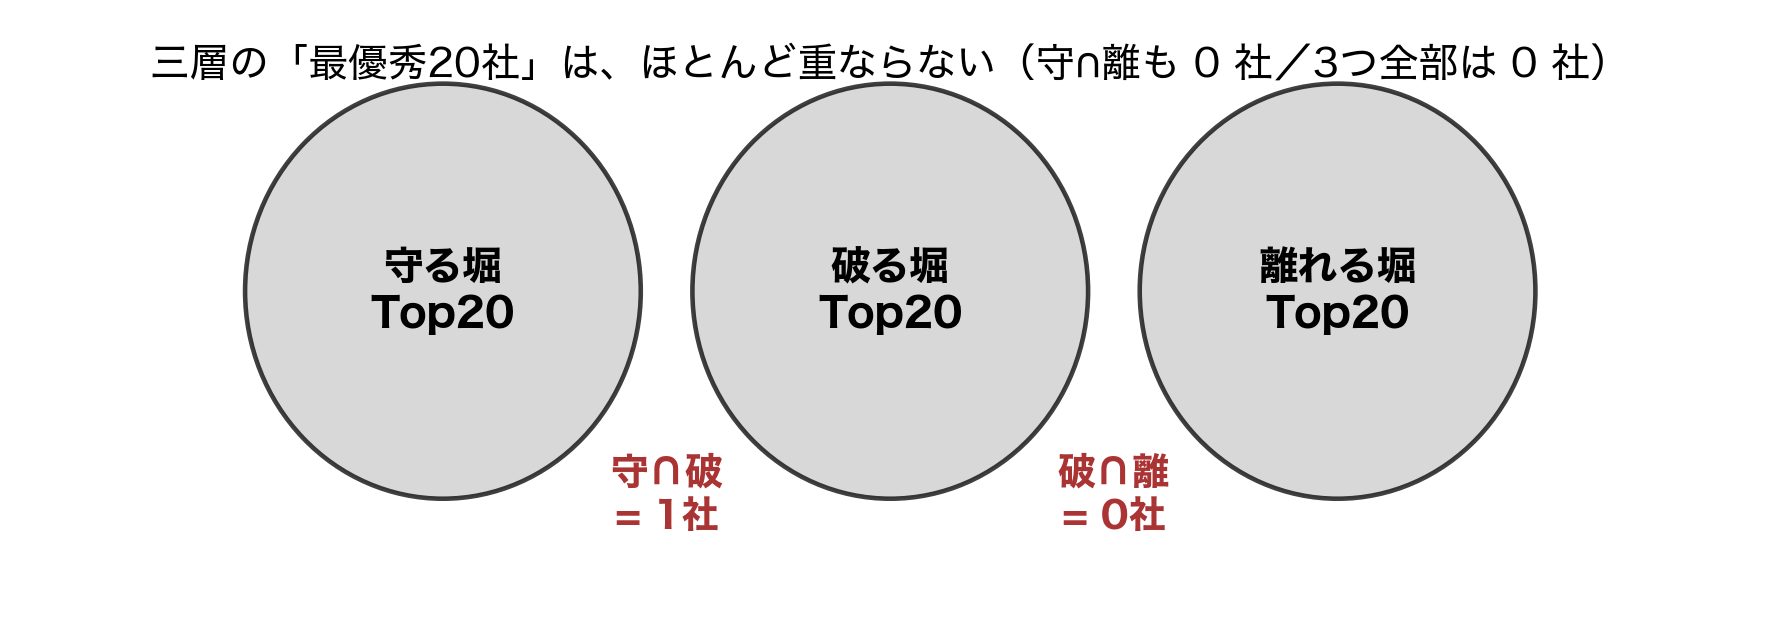
\includegraphics[width=\linewidth]{and_figures/f3_overlap.png}
\caption{各層のトップ20はほとんど重ならない（実測）}
\end{figure}

\begin{center}
\small
\begin{tabular}{lc}
\toprule
組み合わせ & 重なった会社数 \\
\midrule
守る堀トップ20 $\cap$ 破る堀トップ20 & 1社 \\
守る堀トップ20 $\cap$ 離れる堀トップ20 & 0社 \\
破る堀トップ20 $\cap$ 離れる堀トップ20 & 0社 \\
\textbf{3つすべて} & \textbf{0社} \\
\bottomrule
\end{tabular}
\end{center}

考えてみれば当然でもあります。「守る堀」は\textbf{すでに完成して高く評価されている}会社、
「破る堀」は\textbf{まだ安く放置されている}会社です。
高く評価されている会社は安くありません。求めている性質が、そもそも逆向きなのです。

さらに、現行の各層の水準をそのまま3つ重ねると、残るのは\textbf{2社だけ}でした
（6777 santec ＨＤ と 6871 日本マイクロニクス）。20社には遠く及びません。

%=====================================================================
\section{理由③ 業種の壁 ── どんなに緩めても16社が天井}

ここが決定的です。ＡＮＤを通った会社の\textbf{業種が偏る}のです。

理由①で見たとおり、20社を残すにはふるいを「上位22\%」程度まで緩めるしかありません。
ではその状態で本当に20社組めるか。組めません。
なぜなら\textbf{ＡＮＤを通る会社の業種が、最大でも8種類しかない}からです。

「同じ業種は2社まで」というルールのもとで組める最大社数は
$2 \times 8 = 16$。\textbf{20社に4社足りません。}

\begin{figure}[h]
\centering
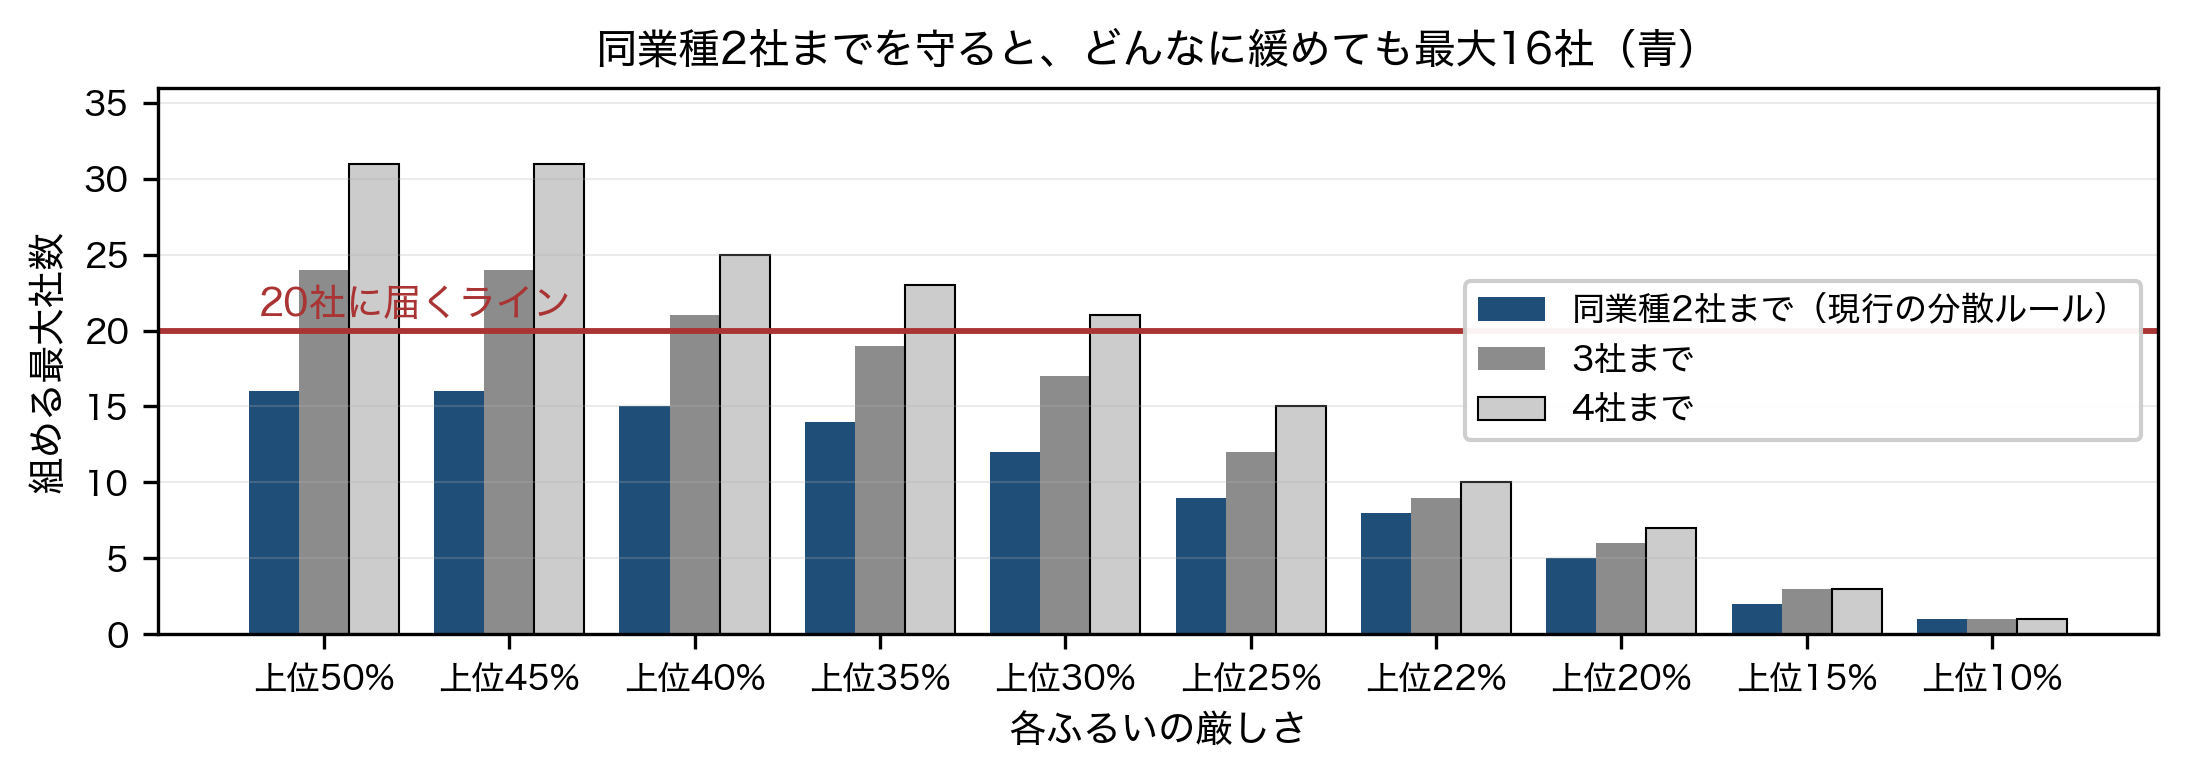
\includegraphics[width=\linewidth]{and_figures/f4_sector_ceiling.png}
\caption{青（同業種2社まで）は一度も20社のラインに届かない}
\end{figure}

\begin{center}
\small
\begin{tabular}{lrrrrc}
\toprule
各ふるいの厳しさ & 通った社数 & 業種の数 & \multicolumn{2}{c}{組める最大社数} & 20社\\
\cmidrule(lr){4-5}
 & & & 2社まで & 4社まで & 成立?\\
\midrule
上位50\% & 278 & 8 & \textbf{16} & 31 & × \\
上位40\% & 120 & 8 & \textbf{15} & 25 & × \\
上位30\% & 64 & 6 & \textbf{12} & 21 & × \\
上位25\% & 17 & 6 & \textbf{9} & 15 & × \\
上位20\% & 7 & 4 & \textbf{5} & 7 & × \\
上位10\% & 1 & 1 & \textbf{1} & 1 & × \\
\bottomrule
\end{tabular}
\end{center}

一番緩い「上位50\%」──もはやふるいと呼べない水準──でさえ16社です。
\textbf{20社という数と、同業種2社までという分散ルールは、ＡＮＤ方式と両立しません。}

20社に届かせるには、業種上限を\textbf{4社まで}緩める必要があります。
そのときの各ふるいは「上位3割」で、守る堀の本来の水準（ＲＯＥ15\%以上＝上位9\%）よりずっと緩く、
もう「守る堀を通った」とは呼べません。

%=====================================================================
\section{理由④ 3段目のふるいは、会社ではなく業種を見ていた}

これが一番深い問題です。「離れる堀のふるい」が何を判定しているのか、業種ごとに通過率を調べました。

\begin{figure}[h]
\centering
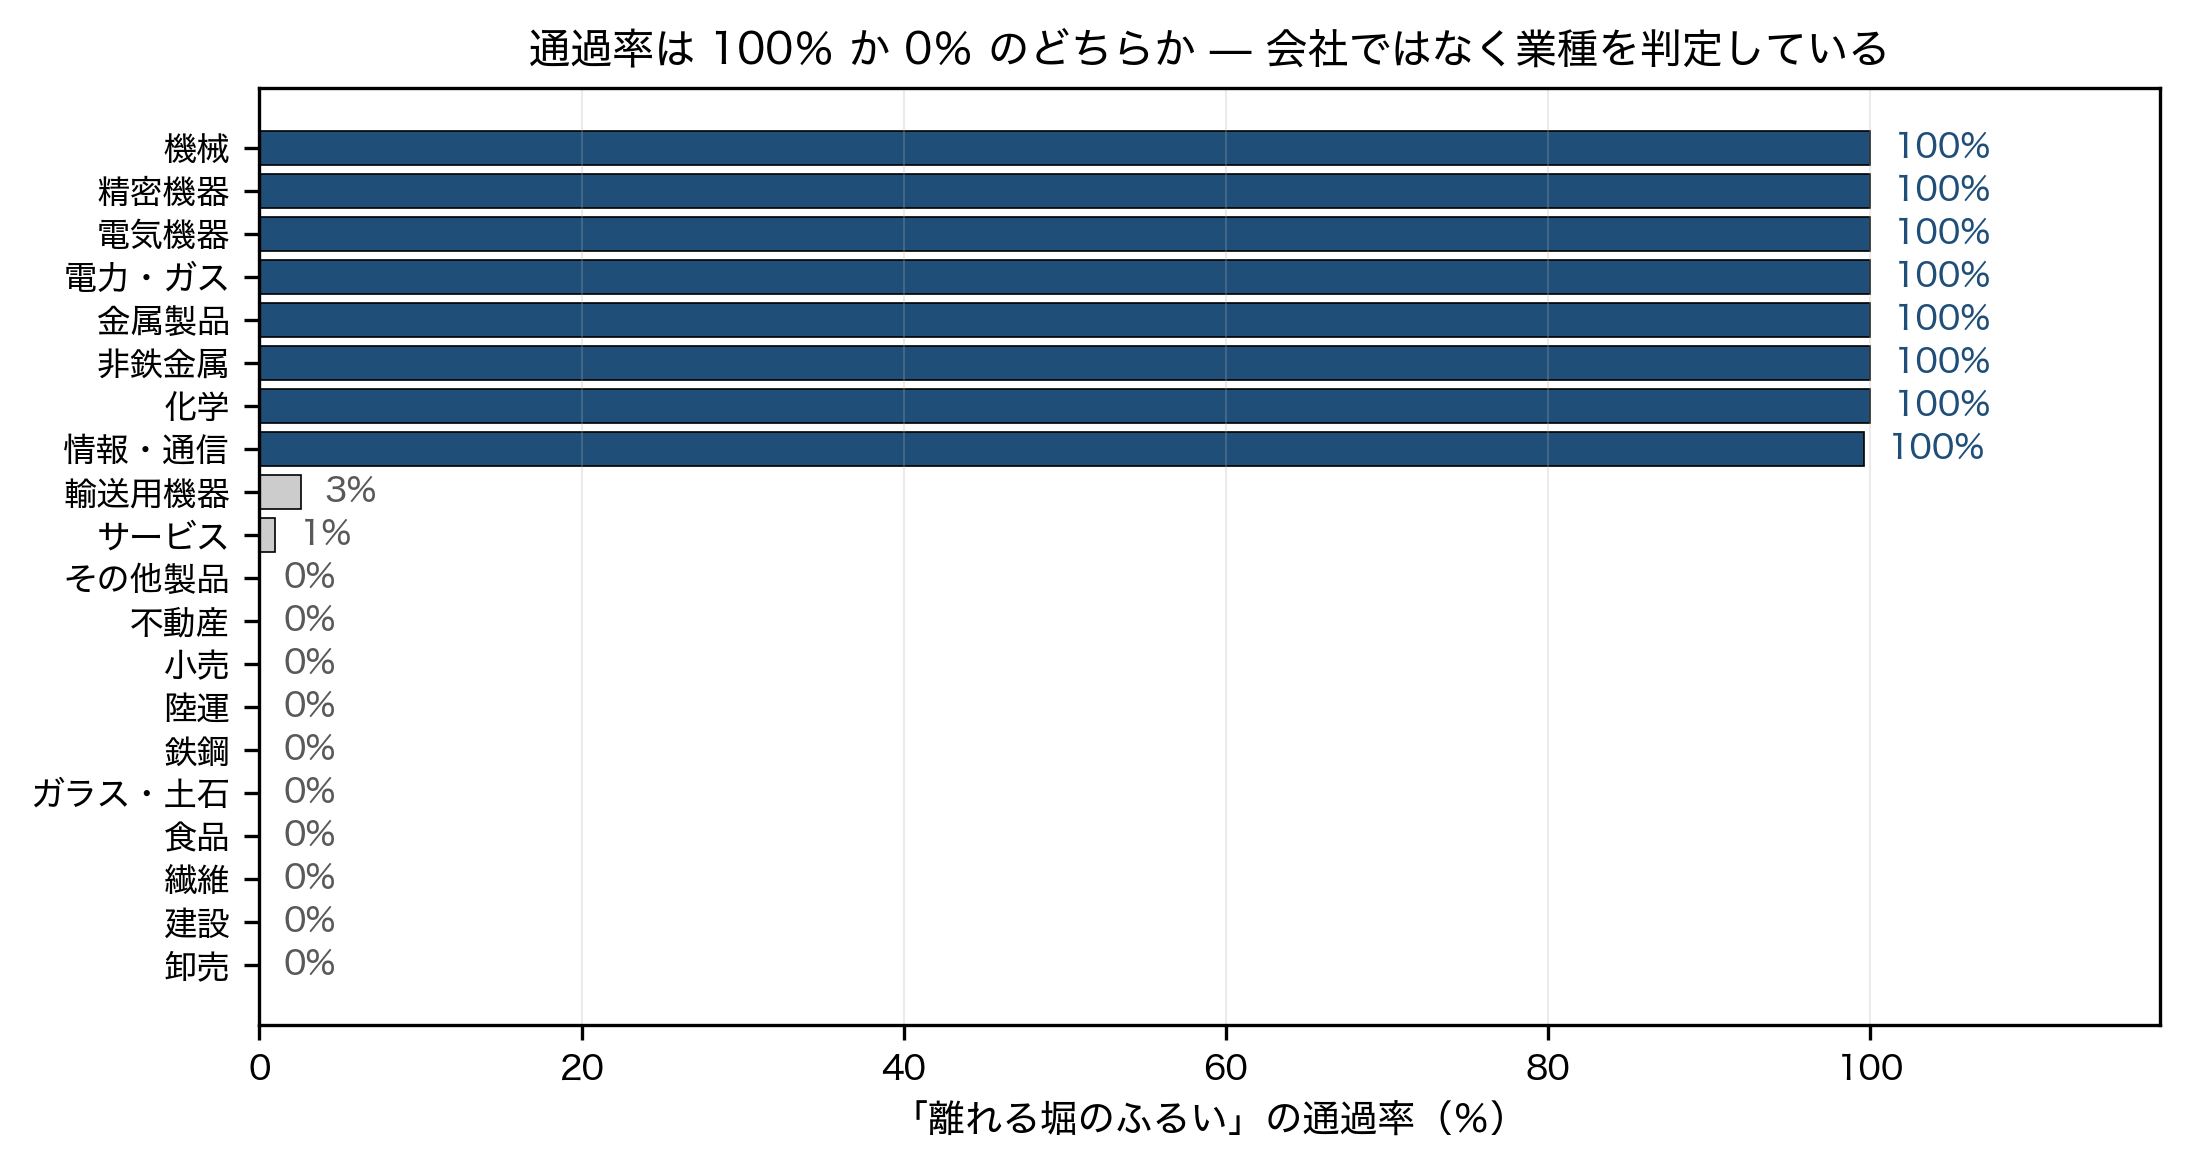
\includegraphics[width=0.93\linewidth]{and_figures/f5_sector_dummy.png}
\caption{通過率が100\%か0\%に割れる。会社の中身では差がついていない}
\end{figure}

機械・精密機器・電気機器・電力ガス・金属製品・非鉄金属・化学は\textbf{通過率100\%}、
情報通信は99.6\%。それ以外の業種は\textbf{ほぼすべて0\%}です。

つまりこのふるいは、会社を選別していません。\textbf{「この8業種に属しているか」を判定しているだけ}です。
原因は、点数の計算で\textbf{業種名に一致すると自動で加点される}仕組みが入っていること、
そして会社ごとに差がつく唯一の材料（研究開発費の比率）が
3,649社中\textbf{2社}しかデータを持たず、残りが0で埋められていることです。
結果として、点数は1,791社に対して\textbf{17通りの値しか取らず}、最も多い値には748社が同点で並びます。

\begin{warnbox}
\jt{だから「3つ全部通ったから最強」という論証が成り立ちません。}\\
3段目に、会社を見分ける情報が入っていないのです。
ＡＮＤを通った会社が業種に偏る（理由③の16社の天井）のも、これが直接の原因です。
実際、ＡＮＤを通った77社のうち\textbf{57社が情報・通信}でした。
\end{warnbox}

なお、この点は現在制作中の査読版レポート（v11）で\textbf{すでに開示済み}です。
「既製のＡＩ関連スコアは企業を並べられない、算術的には業種のラベルだった」と本文に書いてあります。
つまり私たちはこの弱点を知っていて、\textbf{だからこそ}離れる堀の選定を
「点数の並べ替え」ではなく「事業セグメントの開示まで遡って実需を確認する」方式に切り替えました。
ＡＮＤ方式は、いったん捨てたはずの弱い点数に、選定の3分の1を任せ直すことになります。

%=====================================================================
\section{それでも20社組んで、成績を測ってみた}

理屈だけでは納得しにくいので、実際に組みました。
業種上限を4社まで緩めて、ＡＮＤで20社を組み、現行の20社と同じ規約で比べます。

\begin{figure}[h]
\centering
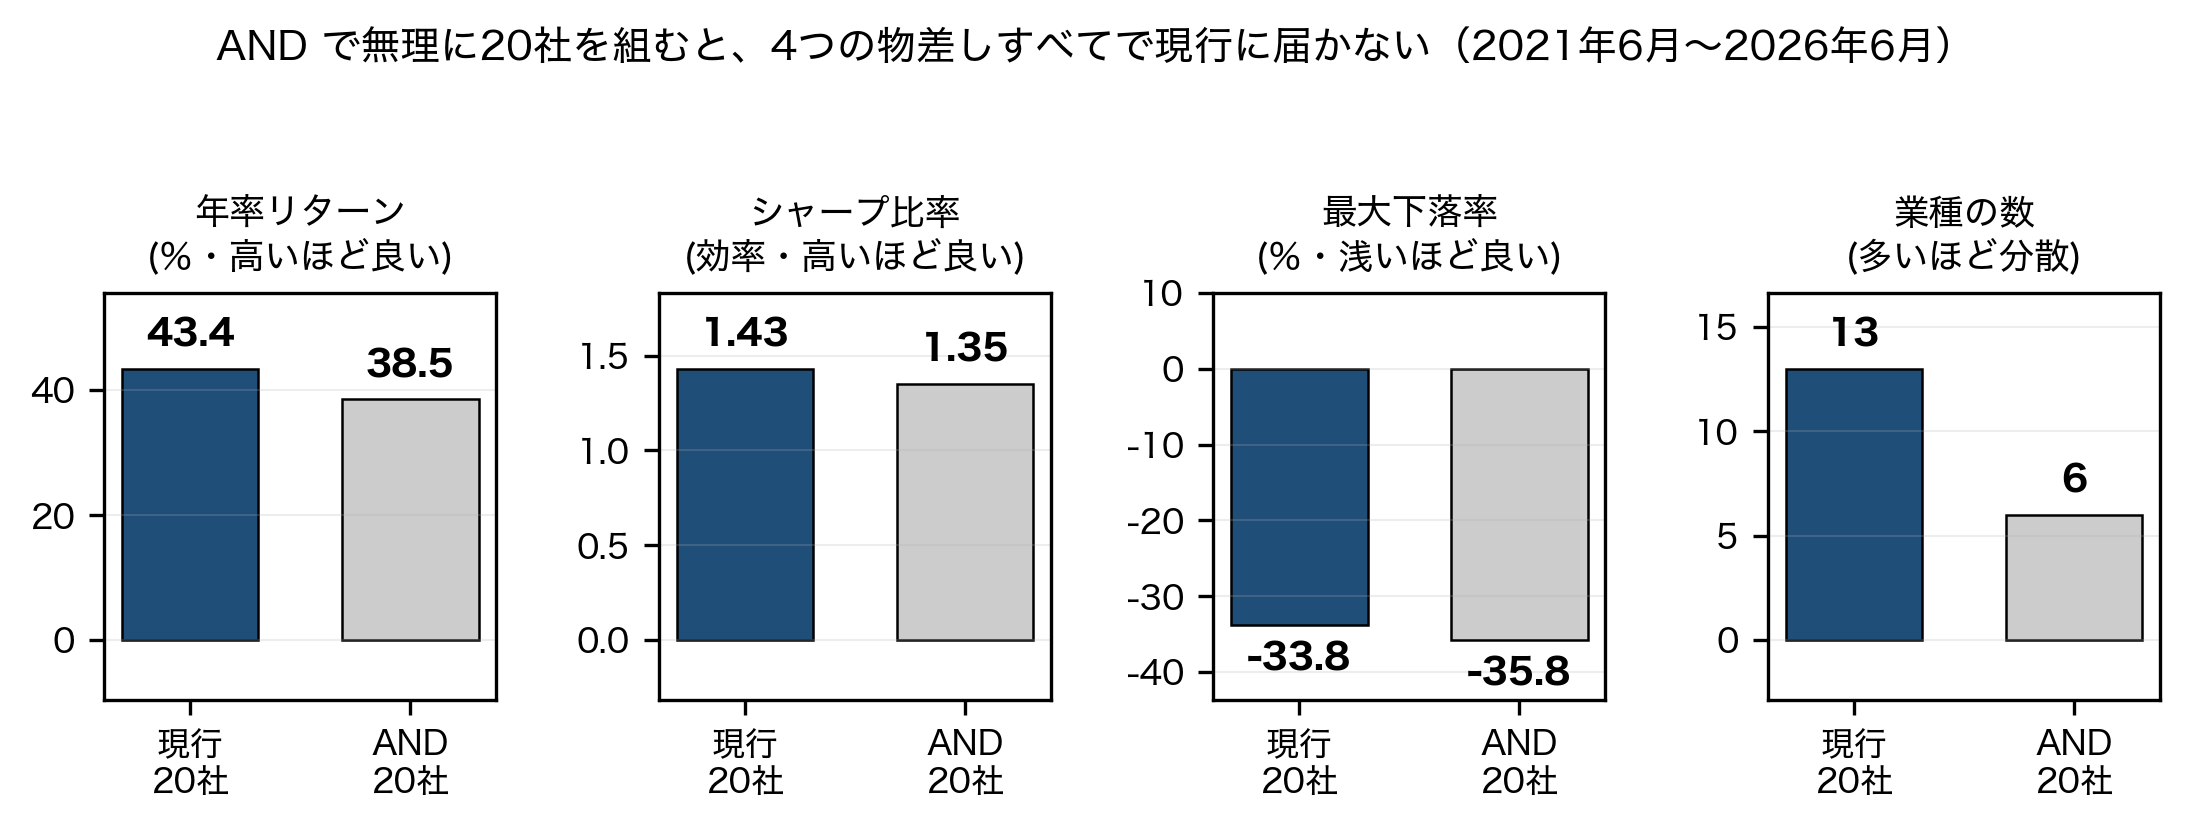
\includegraphics[width=\linewidth]{and_figures/f6_result.png}
\caption{2021年6月〜2026年6月の実測（同じ計測規約・同じ期間）}
\end{figure}

\begin{center}
\small
\begin{tabular}{lccrrrr}
\toprule
選び方 & 20社 & 業種数 & 年率 & シャープ & 最大下落 & 対TOPIX \\
\midrule
\textbf{現行20社（提出版）} & ○ & \textbf{13} & \textbf{43.4\%} & \textbf{1.43} & \textbf{$-$33.8\%} & $+$27.5pt \\
ＡＮＤ・同業種2社まで & \textbf{×(12社)} & 7 & 40.8\% & 1.39 & $-$32.1\% & $+$24.9pt \\
ＡＮＤ・同業種4社まで & ○ & 6 & 38.5\% & 1.35 & $-$35.8\% & $+$22.6pt \\
現行水準のまま3つ重ねる & \textbf{×(2社)} & 1 & 71.0\% & 1.42 & $-$63.5\% & $+$55.1pt \\
3つの点数の合計が良い20社 & ○ & 11 & 28.2\% & 1.24 & $-$25.5\% & $+$12.3pt \\
\bottomrule
\end{tabular}
\end{center}

{\footnotesize
シャープ＝リスク1単位あたりのもうけ（高いほど効率が良い）。最大下落＝期間中いちばん深く落ちた幅（浅いほど良い）。
すべて2026年時点で選んだ20社を過去に当てた自己検証です。\par}

読み取れることは3つあります。

\begin{enumerate}[leftmargin=1.4em,itemsep=2pt]
\item 唯一20社が成立するＡＮＤ版（同業種4社まで）は、\textbf{年率・効率・下落の深さ・業種の分散のすべてで現行に届きません}。
\item 現行水準のまま3つ重ねた版は年率71\%と高く見えますが、\textbf{たった2社}で、最大下落は$-$63.5\%。20社ポートフォリオの代わりにはなりません。
\item 「3つの点数の合計が良い20社」という緩めたＡＮＤも試しましたが、年率28.2\%で最も劣りました。\textbf{満点主義で選ぶと、各層で突き抜けた会社が全部外れる}のです（平均的に良い会社ばかりが残る）。
\end{enumerate}

%=====================================================================
\section{では、提案のねらいはどう活かすか}

提案の本質は「三層の要素を兼ね備えた会社を評価したい」ということでした。
これは\textbf{20社全体の選び方にはできませんが、枠としてすでに入っています}。

\begin{keybox}
現行20社のうち\jt{両立型3社}──6861 キーエンス・7725 インターアクション・6929 日本セラミック──は、
まさに\textbf{「現在の堀」と「未来の堀」の両方の順位が上位}という条件（＝ＡＮＤ）で選ばれた枠です。
黒字・ＲＯＥ5\%以上の1,463社から、両方の順位がともに上位の会社を、業種上限2で選んでいます。

つまり\textbf{「ＡＮＤ的に最強の会社」は、現行20社の中にすでに3社入っています。}
今回の検証が示したのは「ＡＮＤで選べる会社はこの規模しか存在しない」という\textbf{実測に基づく上限}であって、
設計の好みの問題ではありません。
\end{keybox}

チームに返すときは、次の3点を伝えれば提案に正面から答えたことになります。

\begin{enumerate}[leftmargin=1.4em,itemsep=2pt]
\item ＡＮＤを試した。三層のエリートはほとんど重ならない（各層トップ20の重複は0〜1社）。
\item ＡＮＤで20社を組むと各ふるいを上位22\%までしか絞れず（掛け算の必然）、同業種2社までなら最大16社。上限を緩めて組んだ実測は、4つの物差しすべてで現行に劣る。
\item だから「全部入り」は20社の選び方ではなく\textbf{両立型3社という枠}として持ち、残りは役割分担で各層を深く絞る。
\end{enumerate}

%=====================================================================
\section{まとめ（1枚）}

\begin{center}
\small
\begin{tabular}{>{\raggedright\arraybackslash}p{0.30\linewidth}>{\raggedright\arraybackslash}p{0.62\linewidth}}
\toprule
\textbf{理由} & \textbf{実測された事実} \\
\midrule
① 掛け算の壁 &
三つの点数はほぼ無関係（相関$\approx$0）なので、残る社数は$N q^3$。
20社を残すには各ふるいを\textbf{上位22\%}までしか絞れない。「3つ全部でエリート」は要求できない。\\
\addlinespace
② エリートは別人 &
各層トップ20の重複は 守$\cap$破=1社、守$\cap$離=0社、破$\cap$離=0社、\textbf{3つすべて=0社}。
現行水準のまま重ねると\textbf{2社}しか残らない。\\
\addlinespace
③ 業種の壁 &
ＡＮＤを通る業種は最大8種類。同業種2社までなら$2\times8=$\textbf{16社が天井}で、
どの閾値でも20社に届かない。\\
\addlinespace
④ 3段目が業種ラベル &
離れる堀のふるいの通過率は8業種が100\%、他はほぼ0\%。
\textbf{会社ではなく業種を判定している}ので「3つ通ったから最強」が成り立たない。\\
\midrule
\textbf{実測での確認} &
上限4に緩めて20社を組むと、年率38.5\%（現行43.4\%）・シャープ1.35（1.43）・
最大下落$-$35.8\%（$-$33.8\%）・業種6（13）で\textbf{すべて劣位}。\\
\addlinespace
\textbf{活かし方} &
「全部入り」は\textbf{両立型3社}という枠としてすでに存在。ＡＮＤで選べる会社数の上限がそこにある。\\
\bottomrule
\end{tabular}
\end{center}

%=====================================================================
\appendix
\section{付録A ── 用語集}

\begin{termbox}
\begin{description}[leftmargin=6.5em,style=nextline,itemsep=3pt,topsep=1pt]
\item[ＲＯＥ] 自己資本利益率。株主が預けたお金に対して、1年でどれだけ利益を出したか。15\%以上なら優秀。
\item[営業利益率] 売上のうち本業のもうけが何\%か。高いほど価格決定力がある（＝堀が深い）。
\item[自己資本比率] 会社の財産のうち借金でない部分の割合。高いほど財務が丈夫。
\item[割安・ＰＢＲ] 株価が会社の純資産の何倍か。1倍を下回ると「安く放置されている」と見なされる。
\item[相関] 二つの数字の連動の強さ。$+1$で完全に同じ動き、$0$で無関係、$-1$で正反対。
\item[シャープ比率] もうけ$\div$値動きの荒さ。同じもうけなら、値動きが穏やかなほうが高くなる。
\item[最大下落率] 期間中の高値から安値までの下がり幅。浅いほど耐えやすい。
\item[ＴＯＰＩＸ] 東証の株価指数。市場全体の平均としての比較相手。
\item[自己検証] 2026年時点で選んだ20社を、過去の株価に当てて成績を確かめること。
未来を予測できたという主張ではない。
\end{description}
\end{termbox}

\section{付録B ── 数字の出どころと再現方法}

母集団は東証上場3,649社（2026年4月末時点）。
価格は2023年4月25日〜2026年6月1日の日次調整後終値、財務はＥＤＩＮＥＴ提出書類（2026年7月8日取得）。
本資料のすべての数値は、次のスクリプトを実行して再現できます。

\begin{termbox}
{\footnotesize\ttfamily
python3 scripts/and\_feasibility.py \ \ \# 実現可能性の全指標 → and\_feasibility.json\\
python3 scripts/and\_frontier.py \ \ \ \ \# 閾値ごとのフロンティア → and\_frontier.json\\
python3 scripts/and\_backtest.py \ \ \ \ \# 20社を組んで成績比較 → and\_backtest.json\\
python3 scripts/make\_and\_figures.py \ \# 本資料の図6点 → and\_figures/\\
tectonic -X compile AND\_SCREENING\_EXPLAINER\_v1.tex
\par}
\end{termbox}

詳細な検証記録（この資料の元になった正典）は
\texttt{AND\_SCREENING\_FEASIBILITY\_v1.md} にあります。
そこには、本資料で省いた次の内容も含まれます。

\begin{itemize}[leftmargin=1.4em,itemsep=1pt,topsep=2pt]
\item 3つのカテゴリのＡＮＤが定義上0社になる理由（カテゴリは3点数の最大値で1つだけ付ける排他分類のため）
\item 現行20社が各ふるいを何個通っているか（3個通過4社・2個8社・1個8社。現行はＡＮＤポートフォリオではない）
\item 検証の副産物として見つかったデータ欠測の問題（別資料 \texttt{DATA\_MISSINGNESS\_AUDIT\_v1.md} に分離）
\end{itemize}

\vspace{6pt}
{\footnotesize\color{gray}
本資料はすべて in-sample（2026年時点で選んだ銘柄を過去に当てる）の自己検証であり、
リターンはSTOCKリーグの採点対象外です。本資料の目的は提案の実現可能性の判定に限られます。\par}

\end{document}
